\documentclass[11pt]{article}
\usepackage[margin=1in]{geometry}
\usepackage{graphicx}
\usepackage{booktabs}
\usepackage{csvsimple}
\usepackage{array}
\usepackage{hyperref}
\usepackage{tikz}
\usetikzlibrary{positioning}
\hypersetup{colorlinks=true, linkcolor=blue, urlcolor=blue}

% Auto-generated by generate_estimation_assets.py
\newcommand{\EstBestC}{0.10}
\newcommand{\EstFinalThreshold}{0.60}
\newcommand{\EstTrainSize}{281}
\newcommand{\EstCvNSplits}{5}
\newcommand{\EstCvObjective}{f1}
\newcommand{\EstCvSeed}{42}
\newcommand{\EstCvBeta}{n/a}
\newcommand{\EstCvMinPrecision}{0.90}
\newcommand{\EstCvFOne}{0.62}
\newcommand{\EstCvPrecision}{0.75}
\newcommand{\EstCvRecall}{0.61}
\newcommand{\EstCvPrauc}{0.86}
\newcommand{\EstCvRocauc}{0.91}
\newcommand{\EstCvBrier}{0.10}
\newcommand{\EstTestFOne}{0.90}
\newcommand{\EstTestPrecision}{0.90}
\newcommand{\EstTestRecall}{0.90}
\newcommand{\EstTestPrauc}{0.95}
\newcommand{\EstTestRocauc}{0.96}
\newcommand{\EstTestBrier}{0.07}


\title{Layered Guardrails for Faithfulness Detection in Retrieval-Augmented Generation}
\author{Emad Noorizadeh\\Bank of America}
\date{\today}

\begin{document}
\maketitle

\section*{Objective}
This report introduces the layered guardrail stack we deploy to detect and mitigate hallucination in a retrieval-augmented generation (RAG) system. The approach integrates (i) a self-reflective metric prompted directly from the generator, (ii) a distilled classifier that mimics our most capable evaluator LLM, and (iii) a deterministic factual check that verifies atomic claims against retrieved evidence. Together these safeguards elevate the trustworthiness of generated responses while keeping latency compatible with production constraints. To conclude we benchmark the classifier against RAGAS and Galileo to contextualise its performance.

\section{Layered Guardrails Architecture}
The guardrail pipeline is designed so that each layer builds on the signals delivered by the previous one while remaining independently auditable:
\begin{itemize}
  \item \textbf{RAG prompt with self-metric reflection.} A compact reasoning prompt elicits token-level rationales from the generator, scoring its own answer for attribution, confidence, contradiction, answer type, reasoning and utilized evidence. The prompt is optimized to keep the generator on-task, it outputs structured JSON.
  \item \textbf{Answer schema check.} Every response is validated against a strict Pydantic schema that enforces field presence, types, and enumerated values. If validation fails we send a retry prompt that includes the schema errors so the model can self-correct; a configurable max-retry budget prevents infinite loops and triggers error if all retires failed.
  \item \textbf{Distilled faithfulness classifier.} High-quality annotations from a frontier LLM are distilled into a lightweight logistic model served by \texttt{classifier}. Features originate from \texttt{context utilization report} and preserve the instructor's judgment about groundedness, mis-citation, and unsupported entity claims.
  \item \textbf{Deterministic factual check.} A final symbolic pass replays extractive checks (numeric equality, entity cross-referencing, citation coverage). Any failure blocks the answer or triggers human escalation even if the classifier predicts faithfulness.
\end{itemize}

\begin{figure}[ht]
  \centering
  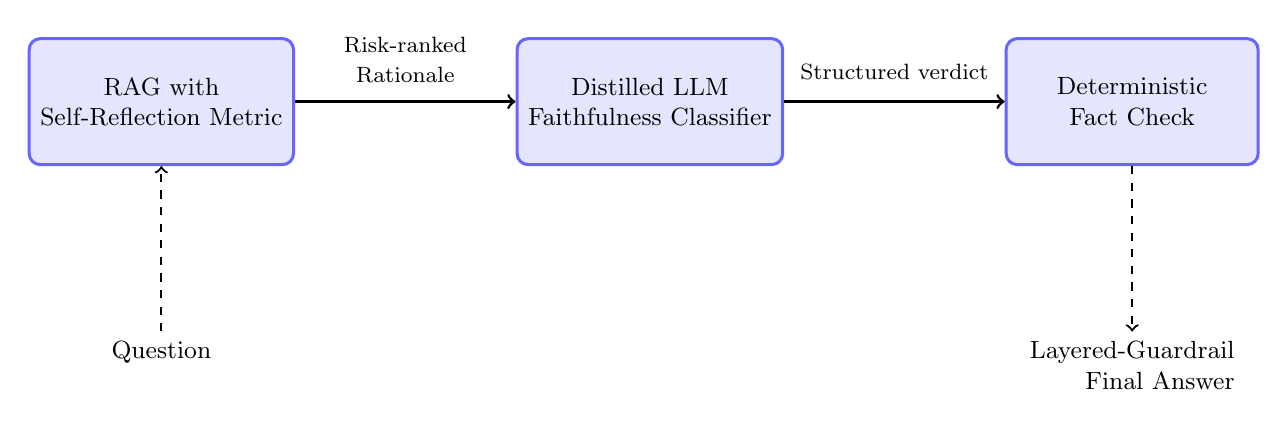
\begin{tikzpicture}[node distance=2.8cm, every node/.style={align=center, font=\small}]
  \tikzset{stage/.style={rounded corners, draw=blue!60, fill=blue!10, line width=1.1pt, minimum width=3.2cm, minimum height=1.6cm, inner sep=4pt}}

  \node[stage] (prompt) {RAG with\\Self-Reflection Metric};
  \node[stage, right=2.8cm of prompt] (classifier) {Distilled LLM\\Faithfulness Classifier};
  \node[stage, right=2.8cm of classifier] (factcheck) {Deterministic\\Fact Check};

  \draw[->, line width=1pt] (prompt) -- node[midway, above=3pt]{\footnotesize Risk-ranked\\\footnotesize Rationale} (classifier);
  \draw[->, line width=1pt] (classifier) -- node[midway, above=4pt]{\footnotesize Structured verdict} (factcheck);

  \node[below=2.1cm of prompt, align=left] (input) {Question};
  \node[below=2.1cm of factcheck, align=right] (output) {Layered-Guardrail\\Final Answer};
  \draw[->, dashed, line width=0.8pt] (input) -- (prompt);
  \draw[->, dashed, line width=0.8pt] (factcheck) -- (output);
\end{tikzpicture}

  \caption{Guardrail stack combining self-reflection, distilled classification, and deterministic fact checking. Dashed arrows visualize the flow from raw generation to the final gated answer.}
\end{figure}

The figure shows how rationales, classifier verdicts, and deterministic proofs compose into a single decision. Each hand-off is logged so that regression tests can replay the path for any example.

\section{Extractor for Faithfulness Signals}
A custom, type-aware extractor was developed specifically for faithfulness detection. It blends deterministic pattern recognizers with optional spaCy fusion to capture grounded entities and inferred values:
\begin{itemize}
  \item \textbf{Normalization.} Numeric mentions are harmonized through unit scaling and ordinal resolution; dates receive timezone-aware parsing; money and percentage formats support variant suffixes. This normalization allows inferred phrasing (for example, ``three quarters'' versus ``75\%'' or ``late Q1'' versus explicit dates) to map onto the canonical entities stored in the index.
  \item \textbf{Entity alignment rules.} Deterministic precedence rules resolve collisions between numeric, monetary, and temporal mentions so a single span cannot double count (e.g., percentages take priority over bare numbers, currency symbols lock a token into MONEY). Cross-field guards ensure DATE parsing does not overwrite numeric quantities and vice versa.
  \item \textbf{Inferred value capture.} Beyond literal string matches, the extractor performs fuzzy harmonization (e.g., company aliases, currency localization) so that the pipeline still recognizes when the answer implies a value missing verbatim from the context but implied by analytics tables.
  \item \textbf{Future calibration.} Index calibration will pre-materialize entity lexicons per document by running a frontier LLM with a tailored entity-prompt over the corpus to enumerate canonical mentions and aliases (people, organizations, products, numerics). The harvested lexicon is versioned and used to seed the extractor so unseen variants are recognized ahead of time, lowering false negatives without widening deterministic regexes.
\end{itemize}

These signals feed \texttt{context utilization report}, where entity and numeric metrics are compared against context spans to produce features such as support ratios, contradiction flags, and hallucination severity scores.

\section{Feature Signals}
The flattened feature space created in \texttt{data\_processing.py} combines lexical, semantic, and structural cues. Each family targets a different failure pattern observed during model audits:
\begin{itemize}
  \item \textbf{Lexical alignment.} These metrics ask whether the retrieved passages even contain the surface form of the answer. They expose unsupported tokens, answer spans that drift beyond the cited context, and retrieval depth issues that correlate with false positives. Key signals include:
    \begin{itemize}
      \item \texttt{best\_context\_share}, per-sentence precision buckets, and unsupported mass ratios for token-level grounding.
      \item Retrieval diagnostics such as \texttt{best\_context\_len} and \texttt{supported\_topk\_impact}.
      \item Question-to-answer coverage measuring how much of the question is satisfied verbatim (or via synonym tables) in the answer.
    \end{itemize}
  \item \textbf{Semantic alignment.} Faithful answers often paraphrase context; these features detect semantic agreement even when literal overlap is low. They also surface suspicious cases where the answer is novel relative to both the context and the question. Key signals include:
    \begin{itemize}
      \item TF--IDF and MiniLM similarities for question-to-answer (\texttt{qr\_alignment.*}) and answer-to-context (\texttt{context\_alignment.*}) pairs.
      \item Novelty and coverage gaps such as \texttt{answer\_novelty\_ratio} and \texttt{qa\_context\_coverage\_gap}.
      \item Per-sentence semantic buckets that flag when embeddings agree despite low lexical overlap.
    \end{itemize}
  \item \textbf{Entity and numeric grounding.} Typed entities and numbers are common hallucination hotspots; these features mirror the deterministic fact check so the classifier can pre-emptively flag unsupported spans. Key signals include:
    \begin{itemize}
      \item Typed entity counts (\texttt{entity\_match.*}, \texttt{supported\_entities.by\_type.*}) and numeric agreement flags.
      \item Unsupported span statistics feeding the deterministic fact check.
    \end{itemize}
  \item \textbf{Inference sensitivity.} Inferred answers (those implied but not explicitly stated) frequently trip the classifier because they resemble hallucinations yet are technically supported. Dedicated inference heuristics lower false negatives by separating confident inferences from true fabrications. Key signals include:
    \begin{itemize}
      \item \texttt{inference\_score}/\texttt{inference\_likely\_bool}: trigger when lexical precision drops below 0.45 but typed grounding (numeric/entity coverage) remains strong and the question-to-answer TF--IDF cosine clears 0.35. The score scales with the lexical gap and typed support so borderline cases stay under the 0.5 threshold.
      \item \texttt{inference\_sem\_score}/\texttt{inference\_sem\_likely}: use MiniLM embeddings to compute a typed-gap ratio (1$-\,$entity support) multiplied by the lexical-to-semantic coverage ratio, flagging situations where embeddings agree even though surface tokens are absent.
      \item \texttt{inference\_explanation}: human-readable rationale that documents why the heuristic fired, aiding review workflows.
    \end{itemize}
  \item \textbf{Discourse and POS markers.} Linguistic cues like hedges, modals, and unsupported head nouns often precede speculative or contradicted statements; incorporating them helps the classifier catch subtle hallucinations that slip past lexical checks. When \texttt{--enable-pos-metrics} is active the pipeline emits:
    \begin{itemize}
      \item Content-word precision and head-noun support rates.
      \item Hedge and modality frequencies that surface speculative phrasing.
    \end{itemize}
  \item \textbf{Signal gap mitigation.} Complementary feature pairs guard against blind spots by measuring the tension between signals. For example, lexical vs. semantic agreement (\texttt{semantic\_gap}) compares context cosine similarity to raw token precision so paraphrased yet grounded answers stay safe. Coverage vs. novelty metrics:
  \begin{center}
  \texttt{qa\_context\_coverage\_gap} \quad \texttt{and} \quad \texttt{answer\_novelty\_ratio}
  \end{center}
  flag answers that introduce new claims. Supported versus unsupported mass, tracked via \texttt{unsupported\allowbreak\_to\allowbreak\_supported\allowbreak\_ratio}, reveals whether the evidence weight still favours grounded spans.\par\smallskip\centerline{\texttt{unsupported\_to\_supported\_ratio}}\par\smallskip In practice, an answer with high lexical precision but a large \texttt{semantic\_gap} combined with elevated \texttt{unsupported\_to\_supported\_ratio} is routed for review—the words match, yet semantics and evidence disagree, signalling a likely hallucination.
\end{itemize}
Across all categories the featurizer currently emits 84 scalar signals, giving the classifier multiple views of each failure pattern. The training script \texttt{k-fold evaluation} ranks features by contribution, while \texttt{feature analyzer} inspects coefficient stability to ensure each signal generalizes across question domains.

\section{Training Dataset}
We curated 3{,}000 diverse question--answer--context triples, labelled by an expert LLM with rationale traces. The data spans financial products, services, tax policies, fees to expose the guardrails to domain shifts. Figure~\ref{fig:train-test-stats} summarizes the train/test split using the CSV derived from the stats exports, while Table~\ref{tab:test-answer-counts} reports the positive answer-type mix recorded alongside those totals.

\begin{figure}[ht]
  \centering
  \renewcommand{\arraystretch}{1.2}
  \csvreader[
    head to column names,
    tabular=>{\raggedright\arraybackslash}p{2.6cm}*{3}{>{\centering\arraybackslash}p{2.2cm}},
    table head=\toprule \textbf{Split} & \textbf{Total} & \textbf{Positive} & \textbf{Negative} \\\midrule,
    late after line=\\,
    table foot=\bottomrule
  ]{files/figure_train_test_stats.csv}{}
  {\Split & \Total & \Positive & \Negative}
  \caption{Train and test label counts generated from the featurization stats. Positives correspond to faithful answers; negatives bundle partially faithful and unfaithful rows.}
  \label{fig:train-test-stats}
\end{figure}

Training rows preserve the self-reflection prompts and rationales so that the distilled classifier can observe both paraphrased admissions of uncertainty and confident but incorrect claims. The validation slice is used for hyper-parameter tuning (regularization, class weights), and the test set stays untouched until final evaluation.

\section{Estimation}
We fit a logistic regression classifier on \EstTrainSize training rows using stratified \EstCvNSplits-fold cross-validation (seeded at \EstCvSeed) to sweep the inverse regularization strength \(C\). The search optimised \texttt{\EstCvObjective} and selected \(C = \EstBestC\) with a decision threshold of \EstFinalThreshold{}. Table~\ref{tab:cv-folds} summarises the per-fold validation metrics; the mean cross-validated F$_1$ was \EstCvFOne{}, with precision/recall of \EstCvPrecision{} and \EstCvRecall{}.

\begin{table}[ht]
  \centering
  \renewcommand{\arraystretch}{1.15}
  \csvreader[
    head to column names,
    tabular=>{\raggedright\arraybackslash}p{1.2cm}*{7}{>{\centering\arraybackslash}p{1.75cm}},
    table head=\toprule \textbf{Fold} & \textbf{F$_1$} & \textbf{Precision} & \textbf{Recall} & \textbf{PR-AUC} & \textbf{ROC-AUC} & \textbf{Brier} & \textbf{Threshold} \\\midrule,
    late after line=\\,
    table foot=\bottomrule
  ]{files/estimation_cv_folds.csv}{}
  {\csvcoli & \csvcolii & \csvcoliii & \csvcoliv & \csvcolv & \csvcolvi & \csvcolvii & \csvcolviii}
  \caption{Cross-validation fold performance at the selected \(C\). Metrics are computed on held-out validation splits.}
  \label{tab:cv-folds}
\end{table}

Final evaluation on the held-out test set achieved F$_1$=\EstTestFOne{}, precision=\EstTestPrecision{}, recall=\EstTestRecall{}, PR-AUC=\EstTestPrauc{}, ROC-AUC=\EstTestRocauc{}, and Brier=\EstTestBrier{}. Table~\ref{tab:test-answer-type} breaks down performance by \texttt{answer\_type}, showing that the distilled classifier maintains recall even on inferred answers.

\begin{table}[ht]
  \centering
  \renewcommand{\arraystretch}{1.15}
  \csvreader[
    head to column names,
    tabular=>{\raggedright\arraybackslash}p{2.8cm}*{5}{>{\centering\arraybackslash}p{1.75cm}},
    table head=\toprule \textbf{Answer type} & \textbf{Support} & \textbf{Precision} & \textbf{Recall} & \textbf{F$_1$} & \textbf{PR-AUC} \\\midrule,
    late after line=\\,
    table foot=\bottomrule
  ]{files/estimation_test_answer_type.csv}{}
  {\csvcoli & \csvcolii & \csvcoliii & \csvcoliv & \csvcolv & \csvcolvi}
  \caption{Held-out test metrics grouped by \texttt{answer\_type}. Empty cells indicate the metric is undefined because only a single class was observed.}
  \label{tab:test-answer-type}
\end{table}

To interpret the fitted model we inspect the largest-magnitude coefficients. Table~\ref{tab:top-features} lists the strongest positive drivers (promoting the faithful class) and the most negative signals (penalising likely hallucinations); these align with the correlation analysis in \texttt{feature\_report.json}.

\begin{table}[ht]
  \centering
  \renewcommand{\arraystretch}{1.1}
  \csvreader[
    head to column names,
    tabular={p{1.9cm}c>{\raggedright\arraybackslash}p{8.4cm}>{\raggedleft\arraybackslash}p{1.5cm}},
    table head=\toprule \textbf{Direction} & \textbf{Rank} & \textbf{Feature} & \textbf{Coeff.} \\\midrule,
    late after line=\\,
    table foot=\bottomrule
  ]{files/estimation_top_features.csv}{}
  {\csvcoli & \csvcolii & \csvcoliii & \csvcoliv}
  \caption{Top logistic-regression coefficients from the distilled classifier. Positive entries boost the faithful class; negative entries suppress it.}
  \label{tab:top-features}
\end{table}

Beyond raw coefficients, the contribution heatmap in Figure~\ref{fig:impact-heatmap} visualises how the same features influence true positives versus false negatives. The horizontal split highlights attributes that support faithful predictions (blue bars) while minimizing pressure in false-negative cases (red bars), providing an at-a-glance diagnostic for feature tuning.

\begin{figure}[ht]
  \centering
  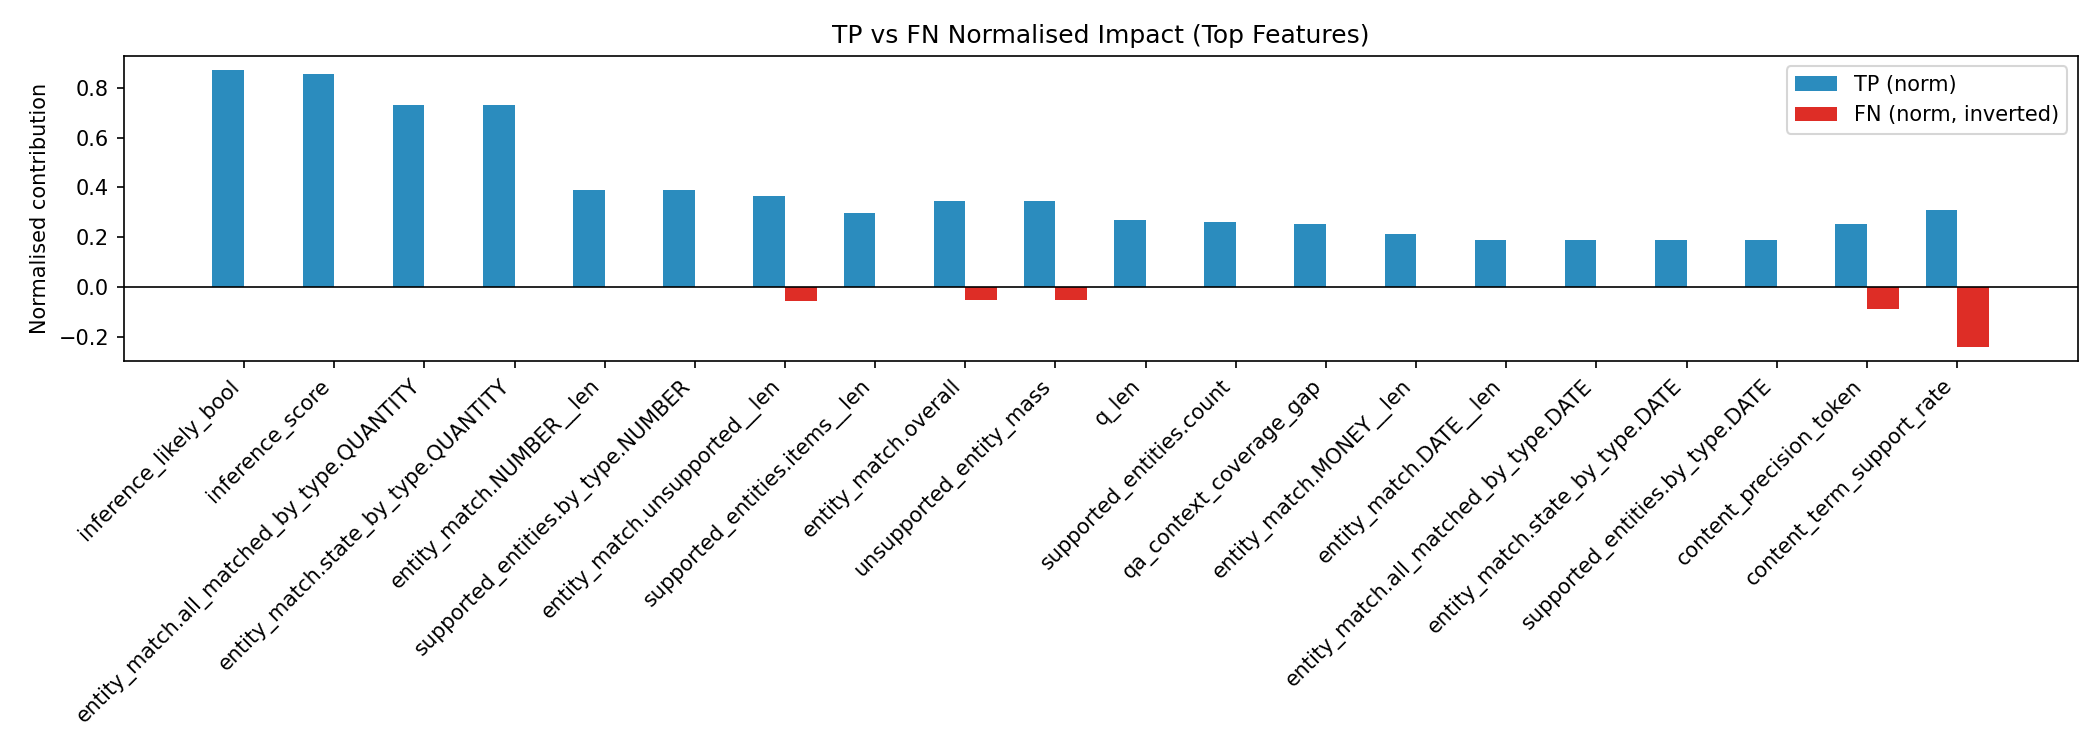
\includegraphics[width=0.82\linewidth]{figs/impact_heatmap_TPFN.png}
  \caption{Feature contribution heatmap comparing normalised support for true positives (blue) against inverted false-negative pressure (red). Generated by \texttt{scripts/analyze\_predictions.py}.}
  \label{fig:impact-heatmap}
\end{figure}

\section{Performance and Benchmarking}
We benchmark the distilled classifier against two widely used evaluation toolkits: RAGAS, an open-source metric suite, and Galileo's commercial guardrail. All three systems score the identical held-out test set summarised in Table~\ref{tab:test-answer-type}. Table~\ref{tab:benchmark} reports precision/recall/F$_1$; our distilled model maintains the strongest balance and outperform others in this dataset.

\begin{table}[ht]
  \centering
  \renewcommand{\arraystretch}{1.2}
  \csvreader[
    head to column names,
    tabular={>{\raggedright\arraybackslash}p{4.2cm}*{3}{>{\centering\arraybackslash}p{2.2cm}}},
    table head=\toprule \textbf{System} & \textbf{Precision} & \textbf{Recall} & \textbf{F$_1$} \\\midrule,
    late after line=\\,
    table foot=\bottomrule
  ]{files/performance_benchmark.csv}{}
  {\csvcoli & \csvcolii & \csvcoliii & \csvcoliv}
  \caption{Benchmark comparison on the held-out test set. The distilled classifier uses the features described in Section~\ref{tab:cv-folds}; RAGAS and Galileo scores come from running their default configurations on the same examples.}
  \label{tab:benchmark}
\end{table}

\begin{table}[ht]
  \centering
  \renewcommand{\arraystretch}{1.15}
  \csvreader[
    head to column names,
    tabular={>{\raggedright\arraybackslash}p{4.0cm}*{4}{>{\centering\arraybackslash}p{2.0cm}}},
    table head=\toprule \textbf{Answer type} & \textbf{Support} & \textbf{Precision} & \textbf{Recall} & \textbf{F$_1$} \\\midrule,
    late after line=\\,
    table foot=\bottomrule
  ]{files/estimation_test_answer_type.csv}{}
  {\csvcoli & \csvcolii & \csvcoliii & \csvcoliv & \csvcolv}
  \caption{Classifier performance by \texttt{answer\_type} on the held-out test set. Empty cells indicate the metric was undefined because only a single class was observed.}
  \label{tab:test-answer-counts}
\end{table}

\section{Inference Workflow}
To keep inference behaviour consistent with training, the online pipeline replays the identical featurisation recipe:
\begin{enumerate}
  \item Run \texttt{data\_processing.py} with the calibrated extractor settings (e.g., \texttt{--use-spacy-fusion}, \texttt{--enable-pos-metrics}) so raw traces receive the same normalisation and entity typing used during training.
  \item Reconcile the produced feature vector with \texttt{featurization\_meta.json}, inserting zero-filled placeholders for any missing columns to preserve the classifier's expected ordering.
  \item Score the aligned vector with \texttt{classifier.py} or \texttt{predict\_batch.py}, then enforce the deterministic fact check via the helper routines in \texttt{metric\_utils.py} before emitting the final verdict.
\end{enumerate}
This mirroring ensures that feature filtering, metadata, and configuration flags remain embedded in the deployed model and remain drift-free over time.

\section{Next Steps}
Future work centres on richer evidence calibration and stronger recall on inferred answers:
\begin{itemize}
  \item Expand the index-calibration job so each document contributes a curated alias lexicon, phonetic hashes, and confidence priors that feed the deterministic checker.
  \item Integrate an entailment-aware module (e.g., a BART-based classifier) to recover borderline false negatives where the answer is implied rather than quoted verbatim.
\end{itemize}

\end{document}
